%Fiquemos com Deus e Nossa Senhora!
%Sao Jose de Cupertino rogai por nos!!
%Honra teu pai e tua mãe!
% ### Uses XeLaTeX ### %
% ### Needs beamer-master ### %
\documentclass[aspectratio=169]{beamer} %. Aspect Ratio 16:9

\usetheme{AI2} % beamerthemeSprace.sty
\usepackage[portuguese]{babel}
\usepackage[utf8]{inputenc}
\usepackage[T1]{fontenc}
\usepackage{ragged2e,gensymb}
\usepackage{amsmath,bm}

\DeclareMathOperator*{\argmin}{arg\,min}
\DeclareMathOperator*{\argmax}{arg\,max}
\DeclareMathOperator{\sign}{sgn}

% DATA FOR FOOTER
\date{2021}
\title{- Máquinas de Boltzmann Restritas}
\author{João Paulo Papa}
\institute{Advanced Institute for Artificial Intelligence (AI2)}

\begin{document}
% ####################################
% FIRST SLIDE 						:: \SliTit{This is the Title of the Talk}{A. B. Name}{Sprace}
% SUB-TITLE SLIDE 					:: \SliSubTit{<title>}{<explanation}
% SUB-SUB-TITLE SLIDE				:: \SliSubSubTit{<title>}{<explanation}
% SLIDE WITH TITLE 					:: \SliT{Title}{Content}
% SLIDE NO TITLE 						:: \Sli{Content} 
% SLIDE DOUBLE COLUMN WITH TITLE 	:: \SliDT{Title}{First Column}{Second Column}
% SLIDE DOUBLE COLUMN NO TITLE 		:: \SliD{First Column}{Second Column}
% SLIDE ADVANCED WITH TITLE 			:: \SliAdvT{Title}{Content}
% SLIDE ADVANCED NO TITLE 			:: \SliAdv{Content}
% SLIDE ADVANCED DOUBLE WITH TITLE 	:: \SliAdvDT{Title}{First Column}{Second Column}
% SLIDE ADVANCED DOUBLE NO TITLE 	:: \SliAdvD{First Column}{Second Column}
% SLIDE BLACK						:: \Black{ <Content> }
% SLIDE WHITE						:: \White{ <Content> }
% ITEMIZATION 						:: \begin{itemize}  \iOn{First} \iTw {Second} \iTh{Third} \end{itemize}
% COMMENT TEXT				 		:: \note{<comment>}
% SECTION 							:: \secx{Section} | \secxx{Sub-Section}
% BOLD SPRACE COLOR				:: \bfs{<text>}
% TABLE OF CONTENT					:: \tocitem{<title>}{<content>}
% LEFT ALIGN EQUATION				:: \begin{flalign*}  & <equation> &   \end{flalign*}
% CENTER ALIGN EQUATION	S			:: \begin{gather*} <equations>  \end{gather*}
% SLASH								:: \slashed{<>}
% BAR								:: \barr{<letter>} instead of \bar{<letter>}
% THEREFORE						:: use \portanto (larger and bold}
% 2 or 3 MATH SYMBOLS				:: \overset{<up>}{<down>} &  \underset{<below>}{\overset{<above>}{<middle>}}  
% INSERT TEXT IN FORMULA			:: \ins{<text>}
% EXERCISE							:: \exe{<exercise #>}{<exercise text>}
% SUGGESTED READING BOX			:: \sug{<references>}
% CITATION							:: \cittex{<citation>}
% CITATION DOUBLE COLUMN 			:: \cittexD{<citation>}
% TEXT POSITION						:: \texpos{<Xcm>}{<Ycm>}{<text>} origin = center of slide : x right | y down
% REFERENCE AT BOTTOM  S/D SLIDE		:: \refbotS{<reference>} \refbotD{<reference>}
% HIDDEN SLIDE						:: \hid
% COLOR BOX 						:: \blu{blue} + \red{rec} + \yel{yellow} + \gre{green} + \bege{beige}
% FRAME 							:: \fra{sprace} \frab{blue} \frar{red} + \fray{yellow} + \frag{green}		
% FIGURE 							:: \img{X}{Y}{<scale>}{Figure.png} 
% FIGURE							:: \includegraphics[scale=<scale>]{Figures/.png}
% FIGURE DOUBLE SLIDE NO TITLE		::  \img{-4}{0.5}{<scale>}{Figure.png} % Image 1st half
%									::  \img{4}{0.5}{<scale>}{Figure.png} % Image 2nd half
% FIGURE DOUBLE SLIDE WITH TITLE		::  \img{-4}{0}{<scale>}{Figure.png} % Image 1st half
%									::  \img{4}{0}{<scale>}{Figure.png} % Image 2nd half
% INCLUDING SWF (Flash)				:: \usepackage{media9} and \includemedia >> USE ACROBAT <<
%%%%%%%%%%%%%%%%%%%%%%%%%%%%%%%%%%%%%%%%%%%%%%%%%%
% ###############################################################################
% FIRST SLIDE
\SliTit{{\LARGE Máquinas de Boltzmann Restritas}}{Advanced Institute for Artificial Intelligence -- AI2}{https://advancedinstitute.ai}
%%%%%%%%%%%%%%%%%%%%%%%%%%%%%%%%%%%%%%%%%%%%%%%%%%
% ###############################################################################
% SLIDE SUB-TITLE
%\SliSubTit{Sub-Title}{Description}{}
%%%%%%%%%%%%%%%%%%%%%%%%%%%%%%%%%%%%%%%%%%%%%%%%%%
% ###############################################################################
%\SliSubSubTit{Sub-Sub-Title}{Description}
 %%%%%%%%%%%%%%%%%%%%%%%%%%%%%%%%%%%%%%%%%%%%%%%%%%


\SliT{Introdução}{

\justifying As Máquinas de Boltzmann Restritas, do inglês \emph{Restricted Boltzmann Machines} (RBMs) são técnicas baseadas no aprendizado de modelos de \textbf{energia}. Elas podem atuar nas etapas de:

\begin{itemize}
	\item Redução de dimensionalidade.
	\item Aprendizado de características.
	\item Classificação.
	\item Pré-treinamento de redes neurais MLP.
\end{itemize}

}

\Sli{
\justifying RBMs, de maneira geral, são modelos probabilísticos compostos por duas camadas: visível $\bm{v}\in\{0,1\}^m$ (entrada) e escondida $\bm{h}\in\{0,1\}^n$. Enquanto que a camada visível é responsável pela leitura dos dados, a camada escondida mapeia sua distribuição por meio de unidades escondidas (binárias, inicialmente) $h_j$ e uma matriz de peso $\bm{W}\in\mathbb{R}^{m\times n}$ que conecta essas duas camadas.

\begin{figure}[htb]
   \centering
	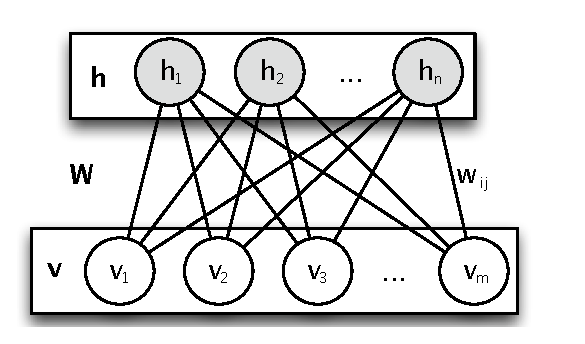
\includegraphics[scale=0.67]{figs/rbm.eps}
	\caption{Arquitetura padrão de uma RBM.}
\end{figure}
}

\Sli{
\justifying Seja ${\cal X} = \{\bm{x}_1,\bm{x}_2,\ldots,\bm{x}_m\}$ um conjunto de dados tal que $\bm{x}_i\in\mathbb{R}^m$. A ideia é aprender os pesos que permitem encontrar o conjunto reconstruído $\hat{{\cal X}} = \{\hat{\bm{x}}_1,\hat{\bm{x}}_2,\ldots,\hat{\bm{x}}_m\}$ a partir da camada escondida $\bm{h}$, em que $\hat{\bm{x}}_i\in\mathbb{R}^m$.

\begin{figure}[htb]
   \centering
	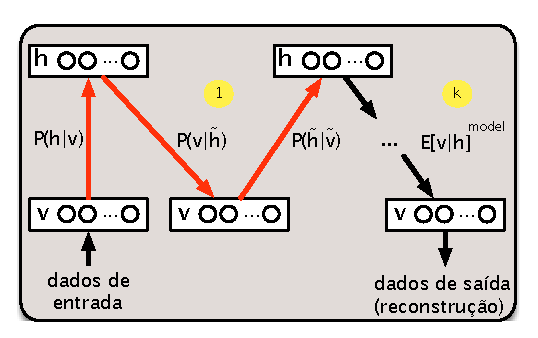
\includegraphics[scale=0.77]{figs/gibbs.eps}
	\caption{Divergência Contrastiva.}
\end{figure}
}

\Sli{

\justifying As seguintes equações podem ser utilizadas para calcular as probabilidades:

\begin{equation}
\label{e.probh}
P(h_j=1|\textbf{v})=\sigma\left(\sum_{i=1}^mw_{ij}v_i+b_j\right),
\end{equation}
e
\begin{equation}
\label{e.probv}
P(v_i=1|\textbf{h})=\sigma\left(\sum_{j=1}^nw_{ij}h_j+a_i\right),
\end{equation}
em que $\sigma(z)=1/(1+\exp(-z))$, $\bm{a}\in\mathbb{R}^m$ and $\bm{b}\in\mathbb{R}^n$ denotam as unidades de bias das camadas visível e invisível, respectivamente, e $w_{ij}\in\mathbb{R}$ corresponde ao peso da conexão entre a unidade (neurônio) visível $i$ e invisível $j$.
}

\Sli{
\justifying De maneira geral, o procedimento de aprendizado de uma RBM consiste em calcular $\textbf{W}$, $\textbf{a}$ e $\textbf{b}$ como segue:
\begin{eqnarray}
\label{e.updateW}
\nonumber \textbf{W}^{t+1}&=&\textbf{W}^t+\eta(E[\textbf{h}\textbf{v}]^{data}-E[\textbf{h}\textbf{v}]^{model})\\
        &=&\textbf{W}^t+\eta(P(\textbf{h}|\textbf{v})\textbf{v}^T-P(\tilde{\textbf{h}}|\tilde{\textbf{v}})\tilde{\textbf{v}}^T),
\end{eqnarray}
e
\begin{equation}
\label{e.updatea}
\textbf{a}^{t+1} = \textbf{a}^t+\eta(\textbf{v}-\tilde{\textbf{v}}),
\end{equation}
e
\begin{equation}
\label{e.updateb}
\textbf{b}^{t+1} = \textbf{b}^t+\eta(P(\textbf{h}|\textbf{v})-P(\tilde{\textbf{h}}|\tilde{\textbf{v}})),
\end{equation}
em que $\textbf{W}^t$, $\textbf{a}^t$ e $\textbf{b}^t$ denotam a matriz de pesos e as unidades de bias para as camadas visível e invisível no tempo $t$, respectivamente.
}

\Sli{
\justifying Posteriormente, novos parâmetros foram introduzidos para melhorar o processo de treinamento: decaimento de peso $\lambda$ e momento $\alpha$. Desta forma, temos novas equações de atualização:

\begin{equation}
\label{e.updateW2}
 \textbf{W}^{t+1}=\textbf{W}^t+\underbrace{\eta(P(\textbf{h}|\textbf{v})\textbf{v}^T-P(\tilde{\textbf{h}}|\tilde{\textbf{v}})\tilde{\textbf{v}}^T)-\lambda\textbf{W}^T+\alpha\Delta\textbf{W}^{t-1}}_{=\Delta\textbf{W}^t},
\end{equation}

\begin{equation}
\label{e.updatea2}
\textbf{a}^{t+1}=\textbf{a}^t+\underbrace{\eta(\textbf{v}-\tilde{\textbf{v}})+\alpha\Delta \textbf{a}^{t-1}}_{=\Delta\textbf{a}^t}
\end{equation}
e

\begin{equation}
\label{e.updateb2}
\textbf{b}^{t+1}=\textbf{b}^t+\underbrace{\eta(P(\textbf{h}|\textbf{v})-P(\tilde{\textbf{h}}|\tilde{\textbf{v}}))+\alpha\Delta \textbf{b}^{t-1}}_{=\Delta\textbf{b}^t}.
\end{equation}
}

\Sli{
\justifying Seja $\bm{\theta}=\{\bm{W},\bm{a},\bm{b}\}$ o conjunto de parâmetros a serem aprendidos durante o processo de reconstrução dos dados e $\bm{\theta}^\ast=\{\bm{W}^\ast,\bm{a}^\ast,\bm{b}^\ast\}$ aquele que minimiza algum critério a ser otimizado (por exemplo, o erro de reconstrução). Temos que a amostragem de Gibbs é muito custosa computacionalmente, muito embora ofereça uma aproximação quase que ideal dos dados de entrada.\newline

\justifying A Divergência Contrastiva, do inglês \emph{Contrastive Learning} (CD), por sua vez, apresenta-se como uma alternativa mais viável. A ideia é utilizar os próprios dados como entrada e algumas poucas iterações para sua reconstrução.
}

\Sli{
\justifying A seguir, mostraremos um exemplo do uso de uma RBM para reconstrução de imagens binárias. O critério de minimização foi o do erro médio quadrático, do inglês \emph{Mean Squared Error} (MSE), entre os pixels da imagem de entrada e da imagem reconstruída. A base de dados a ser adotada é a MNIST, que consiste em imagens de dígitos manuscritos.

\begin{figure}[!ht]
  \centerline{\begin{tabular}{cc}
      	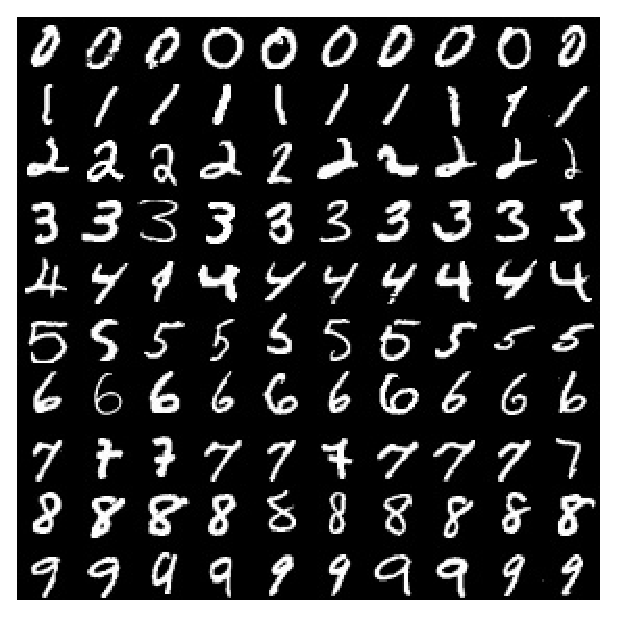
\includegraphics[width=3.1cm,height=3.1cm]{./figs/mosaic_MNdist_dataset.eps} &
      	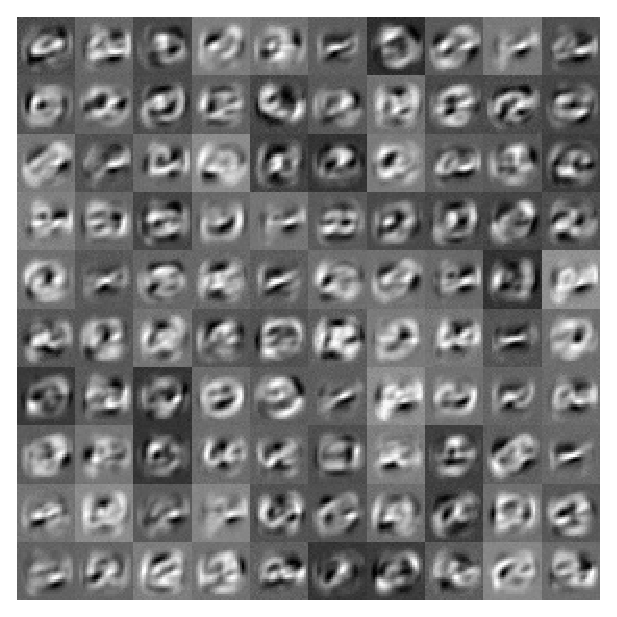
\includegraphics[width=3.1cm,height=3.1cm]{./figs/mosaicMNIST_weights.eps} \\
      	(a) & (b)
\end{tabular}}
\caption{Exemplos de imagens base MNIST: (a) imagens originais e (b) imagens dos pesos da rede.}
\label{f.datasets}
\end{figure}
}

\Sli{
Exemplo de uma RBM treinada apenas com dígitos `0'.
\begin{figure}[!ht]
  \centerline{\begin{tabular}{cccc}
      	\includegraphics[width=1.1cm,height=1.1cm]{./figs/0_10.eps} & 
      	\includegraphics[width=1.1cm,height=1.1cm]{./figs/reconstructed_0.eps} &
      	\includegraphics[width=1.1cm,height=1.1cm]{./figs/1_1133.eps}&
      	\includegraphics[width=1.1cm,height=1.1cm]{./figs/reconstructed_1.eps}\\
      (a) & (b) & (c) & (d)
\end{tabular}}
\centerline{\begin{tabular}{cccc}
      	\includegraphics[width=1.1cm,height=1.1cm]{./figs/weight_1.eps} & 
      	\includegraphics[width=1.1cm,height=1.1cm]{./figs/weight_2.eps} &
      	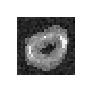
\includegraphics[width=1.1cm,height=1.1cm]{./figs/weight_3.eps}&
      	\includegraphics[width=1.1cm,height=1.1cm]{./figs/weight_4.eps}\\
      (e) & (f) & (g) & (h)
\end{tabular}}
\caption{(a) Dígito original `0'\ e (b) sua reconstrução, (c) dígito `1'\ e (d) sua reconstrução. Alguns pesos da RBM estão mostrados em (e)-(h).}
\label{f.weights}
\end{figure} 
}

\end{document}